%\pgfdeclarelayer{background}
%\pgfdeclarelayer{foreground}
%\pgfsetlayers{background,main,foreground}

% Define a few styles and constants
\tikzstyle{smallbox}=[draw, top color=white, bottom color=blue!20, text width=5em,text centered, minimum height=2.5em]
\tikzstyle{relationship} = [diamond,top color=white,bottom color=red!20,draw=red!50!black!100]
\tikzstyle{bigbox} = [smallbox,top color=white,fill=green!30,minimum height=25em,rounded corners]
\tikzstyle{input} = [coordinate]
\tikzstyle{sum} = [draw, fill=blue!20, circle, node distance=1cm]
\tikzstyle{output} = [coordinate]
\def\blockdist{3}
\def\edgedist{1.5}

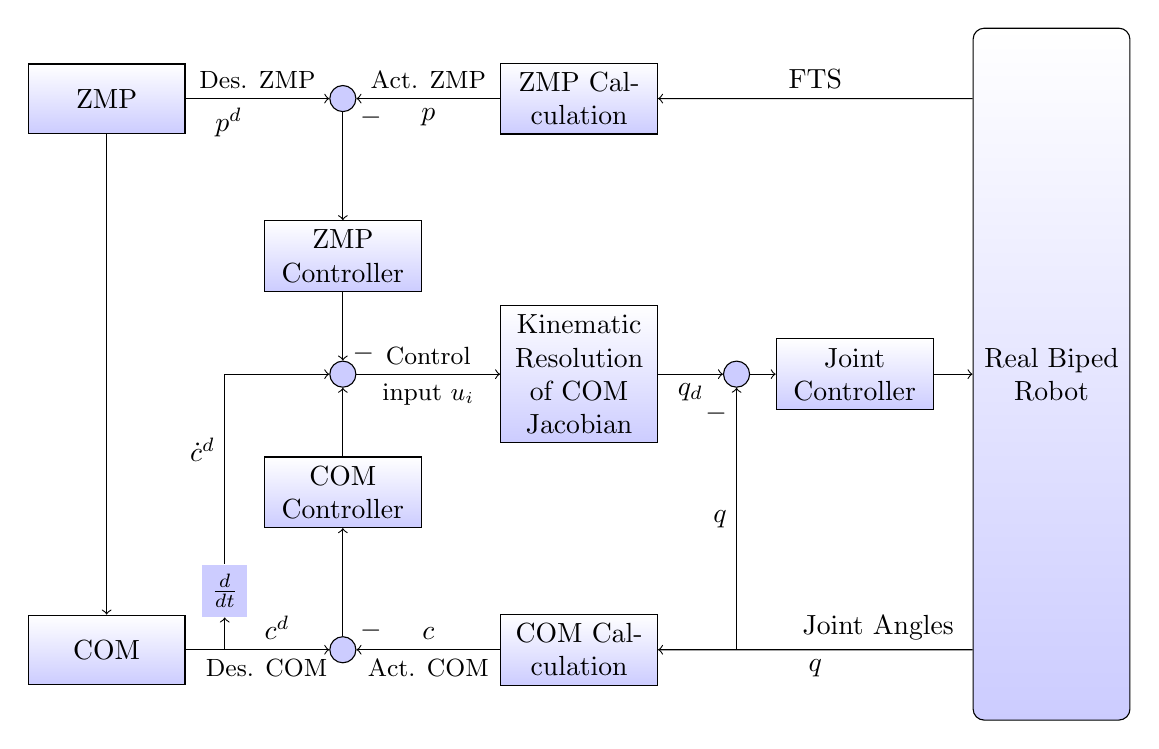
\begin{tikzpicture}[node distance=2cm]
	\node (zmp)[smallbox] {ZMP};
	\node (com) [smallbox,below of=zmp,node distance=7cm] {COM};
	\node (zmp_sum) [sum,right of=zmp,node distance=3cm]{};
	\node (zmp_ctrl) [smallbox,below of=zmp_sum,node distance=2cm]{ZMP Controller};
	\node (ctrl_sum) [sum,below of=zmp_ctrl,node distance=1.5cm]{};
	\node (kin_res) [smallbox,right of=ctrl_sum,node distance=3cm]{Kinematic Resolution of COM Jacobian};
	\node (jnt_sum) [sum,right of=kin_res,node distance=2cm]{};
	\node (jnt_msr) [input,below of=jnt_sum,node distance=3.5cm]{};
	\node (zmp_calc) [smallbox,right of=zmp_sum,node distance=3cm]{ZMP Calculation};
	\node (com_div) [output,right of=com,node distance=1.5cm]{};
	\node (dxdt) [rectangle,fill=blue!20,above of=com_div,node distance=0.75cm]{$\frac{d}{dt}$};
	\node (com_sum) [sum,below of=zmp_sum,node distance=7cm]{};
	\node (com_ctrl) [smallbox,above of=com_sum,node distance=2cm]{COM Controller};
	\node (com_calc) [smallbox,below of=zmp_calc,node distance=7cm]{COM Calculation};
	\node (jnt_ctrl) [smallbox,right of=jnt_sum,node distance=1.5cm]{Joint Controller};
	\node (robot) [bigbox,right of=jnt_ctrl,node distance=2.5cm]{Real Biped Robot};
	
	\draw [->] (zmp) --node[above,pos=0.5]{\small{Des. ZMP}}(zmp_sum)node[below,pos=0.3]{$p^d$};
	\draw [->] (zmp) --node{}(com);
	\draw [-] (com) --node{}(com_div);
	\draw [->] (com_div) --node[below,pos=0.4]{\small{Des. COM}}node[above]{$c^d$}(com_sum);
	\draw [->] (com_calc) --node[below,pos=0.5]{\small{Act. COM}}node[above,pos=0.5]{$c$}node[above,pos=0.9]{$-$}(com_sum);
	\draw [->] (com_div) --node{}(dxdt);
	\draw [->] (com_sum) --node{}(com_ctrl);
	\draw [->] (dxdt) |-node[left,pos=0.3]{$\dot c^d$}(ctrl_sum);
	\draw [->] (com_ctrl) --node{}(ctrl_sum);
	\draw [->] (zmp_ctrl) --node[right,pos=0.9]{$-$}(ctrl_sum);
	\draw [->] (ctrl_sum) --node[above,pos=0.5]{\small{Control}}node[below,pos=0.5]{\small{input }$u_i$}(kin_res);
	\draw [->] (zmp_sum) --node{}(zmp_ctrl);
	\draw [->] (zmp_calc) --node[above]{\small{Act. ZMP}}node[below]{$p$}node[below,pos=0.9]{$-$}(zmp_sum);
	\draw [->] (kin_res) --node[below]{$q_d$}(jnt_sum);
	\draw [->] (jnt_sum) --node{}(jnt_ctrl);
	\draw [->] (jnt_msr) --node[left]{$q$}node[left,pos=0.9]{$-$}(jnt_sum);
	\draw [->] (jnt_ctrl)--node{}(robot);
	\draw [->] (robot.west)+(0,3.5) --node[above]{FTS}(zmp_calc.east);
	\draw [->] (robot.west)+(0,-3.5) --node[above,pos=0.3]{Joint Angles}node[below]{$q$}(com_calc);
	
	\end{tikzpicture}
